\documentclass[10pt]{article}

\usepackage[T2A]{fontenc}
\usepackage[utf8]{inputenc}
\usepackage[english, russian]{babel}
\usepackage{amssymb}

\usepackage{graphicx}
\usepackage{caption}
\usepackage{subcaption}

\newtheorem{theorem}{Theorem}

\title{Синтаксический анализ данных, представленных в виде \\ контекстно-свободной грамматики}
\author{Ковалев Дмитрий Александрович}
\date{}

\begin{document}
	\maketitle
	
	\section{Постановка задачи}
		Целью данной работы является разработка алгоритма синтаксического анализа данных, представленных в виде контекстно-свободной грамматики.
		
		Данная цель приводит к необходимости решения задач, связанных с проверкой пустоты пересечения двух контекстно-свободных языков. Известно, что в общем случае данная проблема неразрешима. В связи с этим, для достижения цели задачи были сформулированы следующим образом.
		
		\begin{itemize}
			\item Изучить существующие подходы к анализу данных, представленных в виде КС-грамматик.
			\item Определить ограничения, при которых синтаксический анализ такого представления является разрешимой задачей.
			\item Разработать алгоритм синтаксического анализа контекстно-свободного представления данных с учетом поставленных ограничений.
			\item Реализовать алгоритм в рамках проекта YaccConstructor.
			\item Доказать завершаемость алгоритма.
			\item Провести тестирование и апробацию.
		\end{itemize}
	
	\section{Обзор}
	
	Пусть $G$ --- произвольная КС-грамматика, $M$ --- конечный автомат. Тогда задача проверки
	\begin{itemize}
		\item включения языков ($L(M) \subseteq L(G)$) --- неразрешима
		\item пустоты пересечения ($L(M) \cap L(G) = \emptyset$) --- разрешима (т.к. в пересечении не более чем КС-язык) за полиномиальное время \cite{Hunt}
		\item регулярности языка $L(G)$ --- неразрешима \cite{Greibach1968}
	\end{itemize} 
	
	Если использовать представление регулярного языка $L(M)$ в виде КС-грамматики $G_r$, то задача проверки пустоты пересечения ($L(G_r) \, \cap \, L(G) = \emptyset$) становится немного интереснее: если $G_r$ 
	\begin{itemize}
		\item нерекурсивная --- задача из PSPACE \cite{Nederhof} (точнее результата нет (я не нашел, по крайней мере))
		\item лево- или праволинейная --- ничего не известно (см. последний абзац заключения из \cite{Nederhof})
		\item принадлежит еще более широкому классу --- тем более ничего не известно
	\end{itemize}
	
	Еще немного про вложенную рекурсию и регулярность языка. Грамматика без вложенной рекурсии (NSE) порождает регулярный язык \cite{Chomsky} (обратное тоже верно, для регулярного языка можно построить NSE грамматику, т.к. праволинейная, например, --- частный случай NSE). Существует алгоритм, который позволяет проверять грамматику на наличие вложенной рекурсии за полином \cite{Anselmo}. Однако, грамматика с вложенной рекурсией тоже может порождать регулярный язык \cite{Andrei2004}, поэтому задача о проверке регулярности языка, порождаемого КС-грамматикой, остается неразрешимой. 
	
	\section{Алгоритм}
	
	Мы пытаемся решать следующую задачу: пусть $G_1 = (N, T, S, P)$ --- произвольная КС-грамматика, $G_2$ --- NSE КС-грамматика. Алгоритм принимает на вход два рекурсивных автомата, $M_1$ и $M_2$, построенных по грамматикам $G_1$ и $G_2$ соотвественно, при этом в автомате $M_2$ левые/правые рекурсивные вызовы заменены на циклы, как в обычном конечном автомате.
	
	Результатом работы алгоритма являются тройки вида $(X, n_1, n_2)$, где $X \in N$, $n_1, n_2$ --- номера состояний автомата $M_2$. 
	Для каждой из таких троек выполняется следующее утверждение: $\exists \, \omega \in T^*$ такая, что $X \rightarrow^* \omega$ в $G_1$ и $\omega \in L(M')$, где $M'$ --- рекурсивный автомат, полученный из $M_2$ путем замены начального и конечного состояния на $n_1$ и $n_2$ соответственно.
	
	Получая такие результаты, мы, по сути, отвечаем на вопрос о проверке пустоты пересечения КС-языка и регулярного, представленных в необычных абстракциях. 
	Для КС-языка мы используем рекурсивный автомат, а для регулярного --- нечто среднее между конечным автоматом и NSE грамматикой (это нечто все еще использует стек, но только для обработки нерекурсивных вызовов). 
	Такое представление эквивалентно по выразительности NSE и, следовательно, FA (см. рис. \ref{circle:lang}). 
	Но неизвестно, к какому классу сложности относится задача (и разрешима ли вообще) о проверке пустоты пересечения регулярного языка, представленного в данной форме, с КС-языком (см. рис. \ref{circle:intersec}).
	
	\begin{theorem}{Завершаемость.}
		Алгоритм завершает работу за конечное число шагов для произвольных входных данных
	\end{theorem}
	
	\begin{theorem}{Корректность.}
		???
	\end{theorem}

	\begin{figure}[h!]
		\begin{subfigure}[t]{0.45\textwidth}
			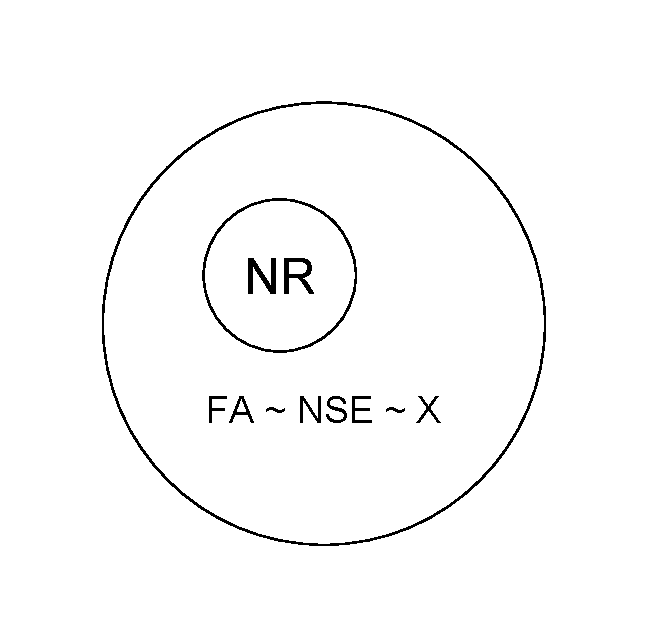
\includegraphics[width=\textwidth]{pictures/lang}
			\caption{Выразительность языка, задаваемого абстракцией}
			\label{circle:lang}
		\end{subfigure}
		~
		\begin{subfigure}[t]{0.45\textwidth}
			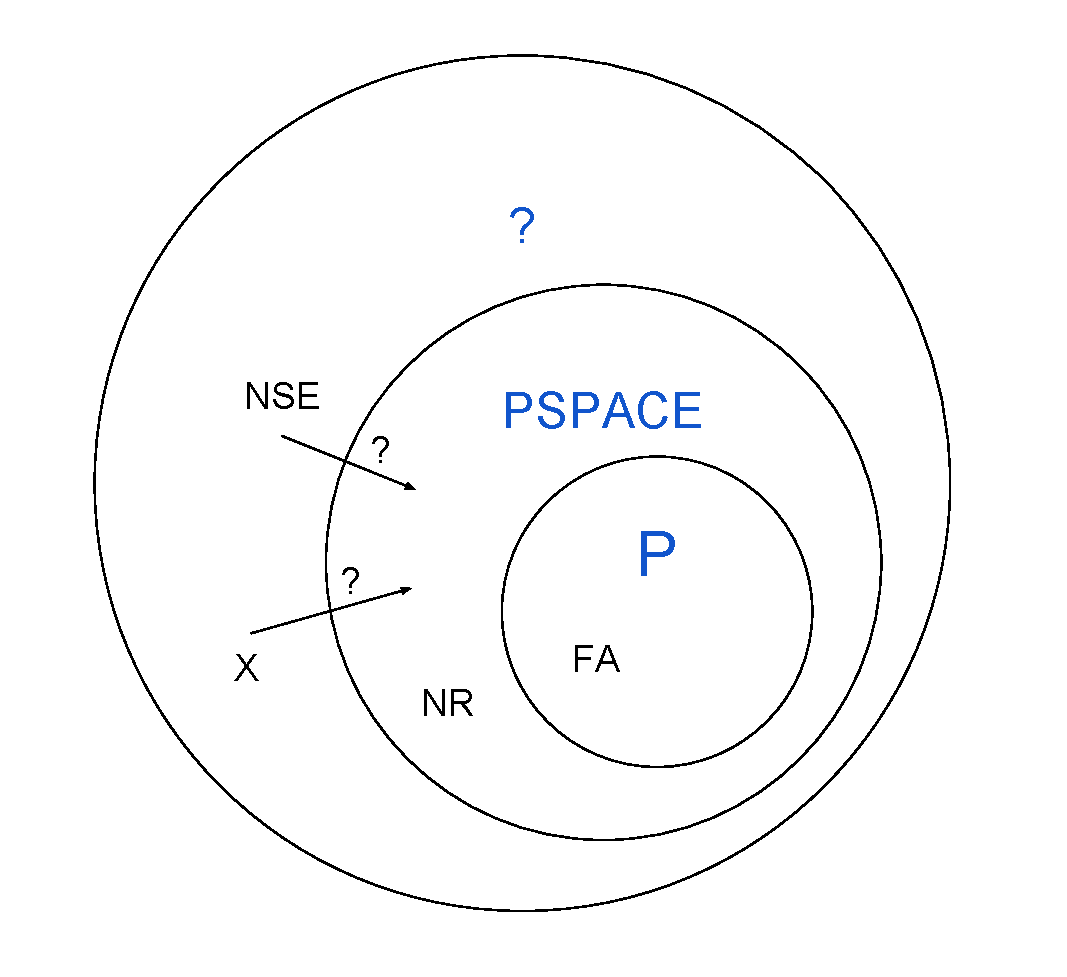
\includegraphics[width=\textwidth]{pictures/intersec_problem}
			\caption{Класс сложности для задачи о проверке пустоты пересечения с КС-языком}
			\label{circle:intersec}
		\end{subfigure}
		\caption{Красивые круги. Здесь NR --- нерекурсивная грамматика, FA --- конечный автомат, NSE --- грамматика без вложенной рекурсии, X --- наше представление}
		\label{circle}
	\end{figure}
	
	\bibliographystyle{abbrv}
	\bibliography{prop}
	
\end{document}